
\chapter{Fazit \& Empfehlung}
In Kapitel xy wurden insbesondere drei Ziele der Arbeit definiert. Diese werden im Folgenden bewertet. 
Die Ergebnisse der Arbeit machen deutlich, welche Schwachstellen und Angriffsvektoren aufzeigen. Aus diesem Grund existiert jedoch nicht bloß eine Alternative. Es gibt verschiedene passwortlose Ansätze, welche sich für verschiedene Anwendungsfälle eignen. Jeder Ansatz hat dabei seine Vor- und Nachteile. Deutlich wird jedoch, dass das FIDO2-Projekt zu den meist untestützten und am weitesten verbreiteten Ansätzen gehört. Dies liegt auch an der gebotenen Vielfalt, da FIDO2 nicht nur Security Keys, sondern beispielsweise auch Passkeys unterstützt.
Im Bezug auf Sicherheit ist das FIDO2-Protokoll eine erhebliche Verbesserung gegenüber der klassischen Passwortauthentifizierung. Da FIDO2 auf öffentliche/private Schlüssel basiert fallen die meisten Angriffsvektoren der klassischen Passwortauthentifizierung weg. 

Aus diesen Gründen empfiehlt sich die Integration von FIDO2 als Alternative ebenfalls für den Unternehmenskontext. Für die Nutzung von Security Keys hingegegen lässt sich keine eindeutige Empfehlung auf den gegebenen Kontext der \ac{LSY} aussprechen. Dies geht vor allem aus den Umsetzungsmöglichkeiten und der erarbeiteten Benutzerfreundlichkeit hervor. Aktuell ist eine FIDO2 Authentifizierung mit Hilfe eines Security Keys noch nicht ausreichend etabliert, um eine gesamte Umstellung vornehmen zu können. Nicht alle Dienste ermöglichen eine FIDO2 Authentifizierung. Zum aktuellen Zeitpunkt eignet sich die Nutzung von Security Keys lediglich für eine \ac{MFA}. Das Ergebnis dieser Arbeit ist allerdings, dass sich die Nutzung von Security Keys insbesondere für eine \ac{SFA} eignet.

Dies entspricht nicht den Richtlinien \ac{SFA}. Solange allerdings keine weitreichende Unterstützung von FIDO2 erfolgt, wird keine Änderung dieser Richtlinie empfohlen. Die Nutzung von Security Keys als zusätzlicher Faktor wird aus wirtschaftlichen Gründen nicht empfohlen. In diesem Fall ist die Nutzung einer Authenticator App besser geeignet.

Grundsätzlich ist eine Nutzung von FIDO2 als Alternative zur klassischen Passwortauthentifizierung zu empfehlen. Sobald eine ausschließliche Nutzung ermöglicht wird lassen siche erhebliche Vorteile für die Sicherheit erzielen. Lediglich die Nutzung von Security Keys ist nicht zweifelsfrei zu empfehlen. In dieser Arbeit werden mehrere Kritikpunkte an der Benutzerfreundlichkeit aufgezeigt. Fragwürdig ist, ob diese Kritikpunkte nach einer erweiterten Gewöhnungsphase noch bestehen. Eine Lösung könnte die Nutzung von Passkeys darstellen. Diese sind allerdings noch nicht weitreichend verbreitet.

Daraus folgt die Empfehlung für die \ac{LSY} nicht direkt auf FIDO2 in Kombination mit Security Keys zu setzen. Stattdessen sollte das Bewusstsein für passwortlose Alternativen erweitert werden. Die Offenheit für Alternativen sollte ebenfalls gefördert. Zusätzlich sollte die Etablierung von FIDO2 weiter beobachtet werden. Sobald eine ausschließliche Nutzung möglich ist, sollte eine Umstellung erfolgen.

\chapter{Ausblick Passkeys}
Ein Problem der Nutzung von FIDO2 mit Hilfe von Security Keys ist die Abhängigkeit an ein einzelnes Gerät. Mit Passkeys stellt FIDO2 eine Alternative, welche multi-device fähige Zugangsdaten ermöglicht \cite{usecasfido}.

Abhängigkeit von Anbietern für beispielsweise Authenticator Apps, welche diese Möglichkeit integrieren müssen. Technisch ist dies mit FIDO2 allerdings schon integriert \cite{usecasfido}.

Erhöhte Benutzerfreundlichkeit gegenüber Security Keys. Keine zusätzliche Hardware notwendig, bzw. möglich mehrere Geräte zu nutzen \cite{usecasfido}.

Vergleichbar wie die Nutzung von auto fill Passwortmanagern, allerdings mit erhöhter Sicherheit und ohne Notwendigkeit von \ac{MFA} \cite{usecasfido} \cite{passkeysgoogle}.

Typischerweise würde die für CTAP2.1 benötigte autorisierung mit Hilfe eines biometrisches Merkmales erfolgen \cite{usecasfido}.

So würde eine Abhängigkeit an die Hardware-Anbieter bestehen. Denn die Sicherheit der Passkeys würde von der Sicherheit der Hardware und des Betriebsystems abhängen, auf welchem die Passkeys gespeichert werden \cite{usecasfido}.

Zusätzlich ermöglicht der FIDO2 Standard die Nutzung von Bluetooth. Dies ermöglicht eine Nutzung von Passkeys mit mobilen Geräten. Dies ist eine Absicherung, falls eine Synchronisierung von Passkeys nicht möglich ist. Dies könnte beispielsweise der Fall sein, wenn Geräte unterschiedlicher Anbieter genutzt werden \cite{usecasfido}.

Dabei kann zusätzlich zum synchronisierten Passkey optional ein Gerätespezifischer Schlüssel erzeugt werden. Der Passkey kann somit nur mit den Geräten genutzt werden, welche einen Gerätespezifischen Schlüssel besitzen \cite{usecasfido}. Dies würde die Sicherheit erhöhen, da die Anbieter der Synchronisierungsdienste keinen Zugriff auf die Passkeys hätten.

Der Google Password Manager ermöglicht bereits eine Synchronisierung der Passkeys und verschlüsselt diese zusätzlich. Der benötigte private Schlüssel für die Verschlüssellung wird dabei lediglich auf dem Gerät selbst gespeichert und ist dort zusätzlich verschlüsselt \cite{passkeysgoogle}.

Zusätzlich ermöglicht dieser auch die Nutzung des Passkeys inklusive eines device-bound Schlüssels. Dieser Schlüssel wird auf Android Geräten auf der \ac{TEE} gespeichert. Somit ist dieser zusätzlich auf der Hardware-Ebene geschützt. Das bedeutet allerdings auch, dass dieser nicht von Backups betroffen ist und nicht wiederherstellbar ist \cite{passkeysgoogle}.

Auch Apple bietet die synchronisierte Nutzung von Passkeys an. Diese werden dabei in der iCloud Keychain gespeichert. Diese ist dabei ebenfalls lediglich in verschlüsselter Form synchronisiert. Eine Möglichkeit zur Nutzung von Passkeys inkluse eines device-bound Schlüssels wird aktuell nicht in der Dokumentation von Apple erwähnt \cite{passkeysapple}.

\begin{figure}[h]
	\centering 
	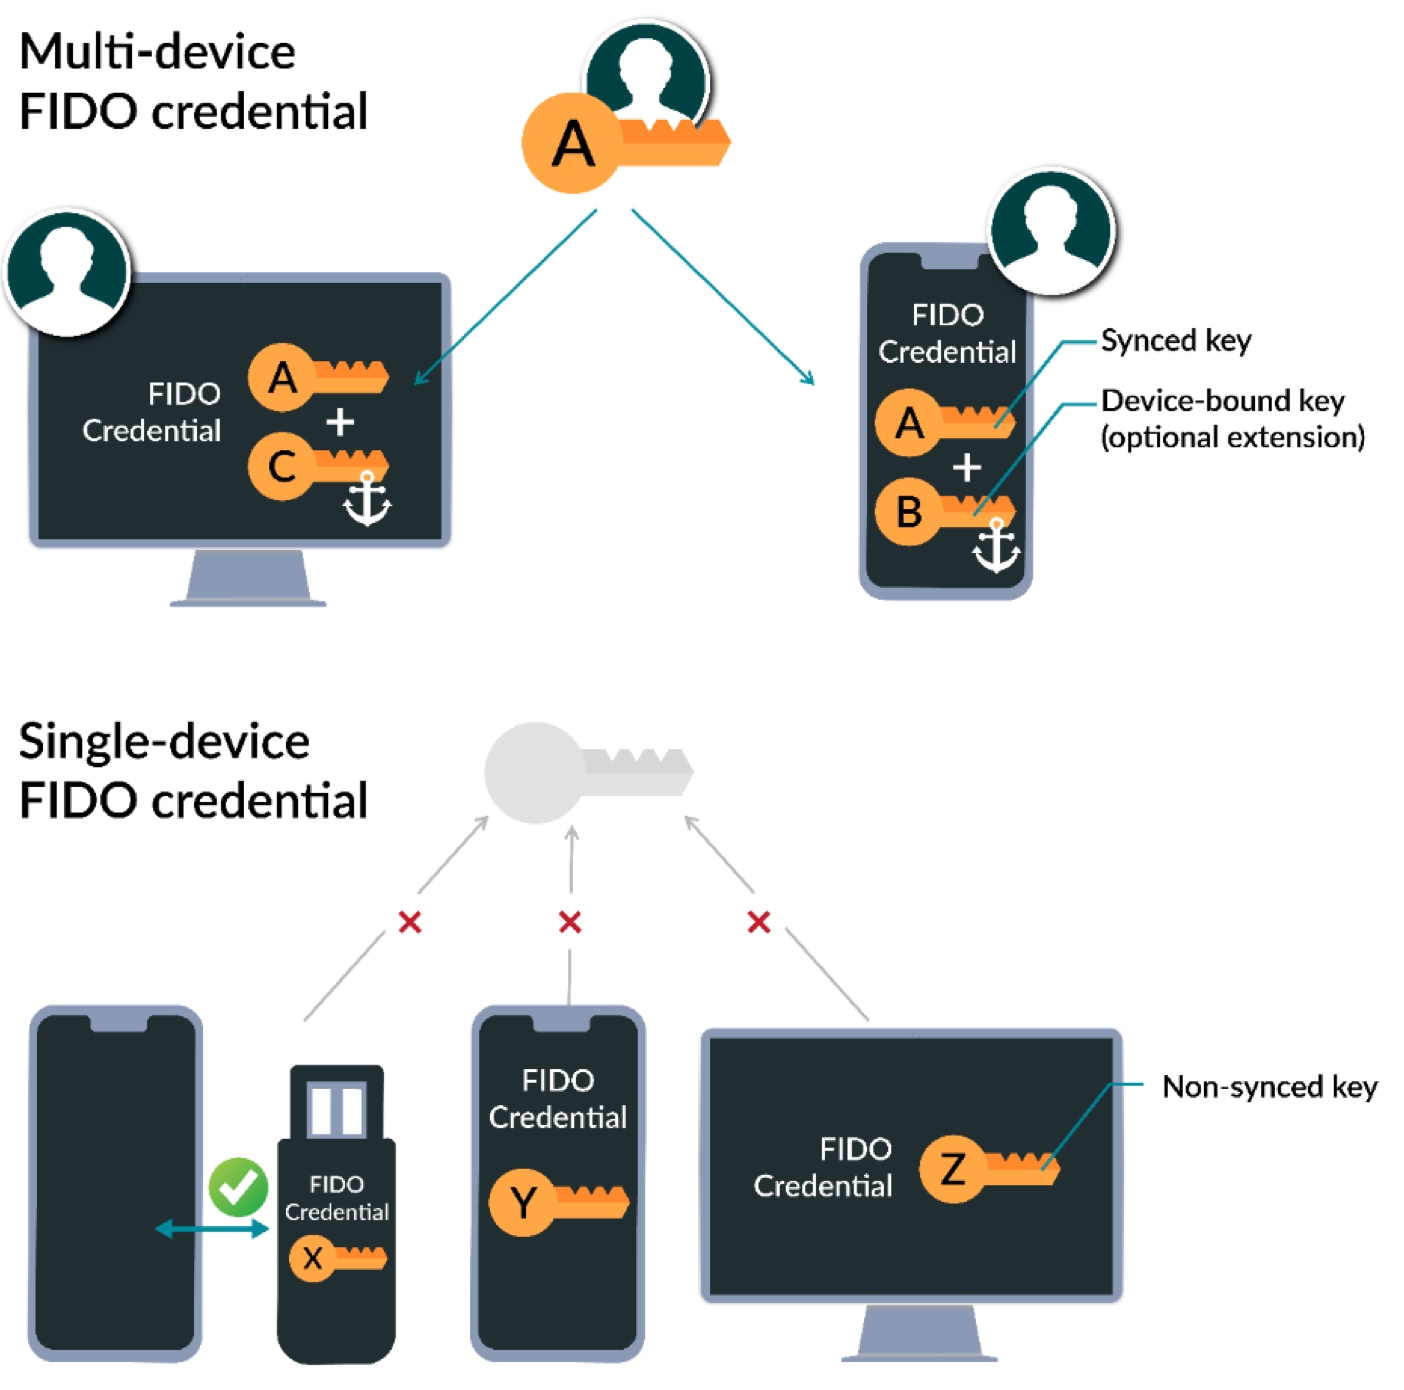
\includegraphics[width=0.7\textwidth]{img/abbildungen/multi-device-fido2.png}
	\captionsetup{format=hang}
	\caption{Multi-device FIDO und Single-device FIDO \cite{usecasfido}} \label{azure-seckey}
\end{figure}





